
%----------------------------------------------------------------------------------------
%	PART
%----------------------------------------------------------------------------------------


\chapter{
	رویکرد پروژه 
}

%----------------------------------------------------------------------------------------
%	CHAPTER 4
%----------------------------------------------------------------------------------------

%\chapterimage{chapter_head_2.pdf} % Chapter heading image
رویکرد پروژه به‌صورت محصول‌محور
\LTRfootnote{Product driven}
خواهد بود. محصول‌محور در مقابل مشتری‌محور 
\LTRfootnote{Customer driven}
مطرح می‌شود و به این معناست که ابتدا محصول طراحی و تولید شده سپس به مسائل مربوط به جذب مشتری، تحلیل متقاضیان و خواسته‌های آن‌ها، جستجوی بازار مناسب و دیگر مسائل مربوط به این دسته پرداخته می‌شود. در حالی که در رویکرد مشتری‌محور ایتدا بازار هدف به صورت دقیق مشخص و شناسایی می‌شود و با مشتریان تعامل صورت می‌گیرد. در این تعاملات، خواسته‌ها و نیازهای مشتریان مشخص شده و محصول مورد نظر برای رفع نیازهای مطرح شده مطرح می‌شود.
رویکرد محصول‌محور ریسک بیشتری دارد چرا که بر این فرض استوار است که محصول نهایی یک حفره را پر خواهد کرد و بازار مناسبی خواهد داشت.

از روش توسعه‌ی چابک نرم‌افزار 
\LTRfootnote{Agile software development}
به عنوان فرایند پیشبرد پروژه استفاده خواهیم کرد. 
این روش مبتنی بر تکرار است. این روش برنامه‌ریزی تطبیقی، توسعه و تحویل تکاملی و رویکرد زمان بسته‌بندی تکرارشونده را ارتقا می‌بخشد و پاسخ‌های سریع و انعطاف‌پذیر برای انجام تغییرات را تقویت می‌کند. این یک روش تدریجی می‌باشد که در آن از حجم طراحی‌های کامل مقدم بر اجرا کاسته شده و طراحی  و اجرا و پیاده‌سازی در بسته‌های کوچک با یکدیگر ادغام شده‌اند. 

مسیر پروژه و تحویل‌دادنی‌ها در هر فاز در زیر آمده‌ است.

\begin{figure}[h]
	\centering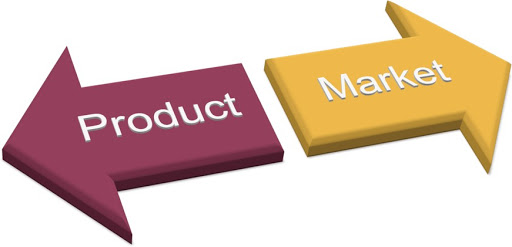
\includegraphics[scale=0.8]{product_vs_customer2}
	\caption{رویکرد پروژه}
	\label{phases} % Unique label used for referencing the figure in-text
	%\addcontentsline{toc}{figure}{Figure \ref{fig:placeholder}} % Uncomment to add the figure to the table of contents
\end{figure}


\section{مسیر پروژه}
پروژه از ۵ فاز کلی تشکیل شده است. ۴ فاز اول مربوط به مراحل تولید بوده و در تلاش برای ایجاد محصول می‌باشد. فاز آخر مربوط به مراحل پس از تولید است و در تلاش برای بهبود محصول موجود می‌باشد.

در فاز اول گستره و مسئله را به‌طور دقیق تعریف می‌کنیم. ایده‌ کلی برای محصول را مطرح کرده و استدلال می‌کنیم که این محصول به چه نیازهایی پاسخ خواهد داد.

در فاز دوم، به تحلیل مسئله 
\LTRfootnote{Problem analysis}
پرداخته و به صورت دقیق حفره‌های موجود را بررسی می‌کنیم. به بررسی نیازمندی‌ها 
\LTRfootnote{Requirement analysis}
می‌پردازیم و مطابق با آن‌ها محصول مورد نظر را به صورت دقیق‌تر طراحی می‌کنیم. در طراحی سیستم این نکته در نظر گرفته می‌شود که رضایت تمام ذی‌نفعان تا جای ممکن تامین شود. بررسی نیازمندی‌ها به جلب رضایت کاربران به عنوان یکی از مهم‌ترین ذی‌نفعان کمک بسیار می‌کند.
در این فاز سناریو‌های سیستم را طراحی می‌کنیم و نمودار مورد کاربرد 
\LTRfootnote{Problem analysis}
را با توجه به نیازمندی‌ها و به روش اصولی به‌دست خواهیم آورد. یعنی ابتدا اکتورها و موردکاربردها و سپس روابط بین آن‌ها را به‌دست خواهیم آورد.

فاز سوم مربوط به مدل‌سازی فرآیندها است. در این مرحله در سطح منطقی 
\LTRfootnote{Logical design}
به طراحی سیستم و فرآیند‌های آن می‌پردازیم، موجودیت‌‌ها را طراحی می‌کنیم، بانک‌های اطلاعاتی را تشکیل می‌دهیم و روابط بین موجودیت‌ها را مشخص می‌کنیم.

فاز چهارم مربوط به پیاده‌سازی و ارزیابی سامانه است. با توجه به طراحی‌ها و مدل‌سازی‌های انجام شده در فازهای قبلی،‌ در قالب فرآیند چابک اسکرام به پیاده‌سازی محصول می‌پردازیم. نکته مهم در این بخش، تداوم و همگامی ارزیابی و پیاده‌سازی است. به این معنا که فرآیند پیاده‌سازی به تعدادی زیربخش تقسیم می‌شود. پس از پایان هر زیربخش، ابتدا عملکرد آن مورد بررسی و ارزیابی دقیق قرار می‌گیرد و در صورت تایید ب مرحله بعدی پیاده‌سازی می‌رویم. این کار در نگاه اول فرآیند پیاده‌سازی را طولانی و زمان‌گیرتر جلوه می‌دهد. اما در نهایت تاثیر به سزایی در بهبود زمان و انرژی مصرف شده خواهد گذاشت. با تقسیم پیاده‌سازی کلی به تعدادی زیربخش، دقت روی هر بخش زیاد شده و ارزیابی دقیقی روی آن صورت می‌گیرد. در این حالت پیدا کردن ایرادات فنی و غیرفنی و برطرف کردن آن‌ها راحت‌تر است. 
نکته دیگر که حائز اهمیت است، تداوم مستندسازی در این فاز است. مستندسازی نیز در نگاه اول به عنوان یک سربار دیده می‌شود اما مستند سازی نقش بسزایی در کاهش هزینه‌های مربوط به نگه‌داری از محصول دارد که در کاهش هزینه‌های نهایی محصول سهم اصلی خواهد داشت.

فاز پنجم مربوط به ارزیابی کلی سامانه به عنوان یک محصول کامل است. حالت کامل این ارزیابی زمانی تحقق می‌یابد که محصول کامل و آماده شده باشد و توسط کاربران (هرچند محدود) استفاده شود.
هدف از این بخش مانیتور کردن عملکرد محصول و اعلام ایرادات احتمالی جهت رفع آن‌ها می‌باشد.

\begin{figure}[h]
	\centering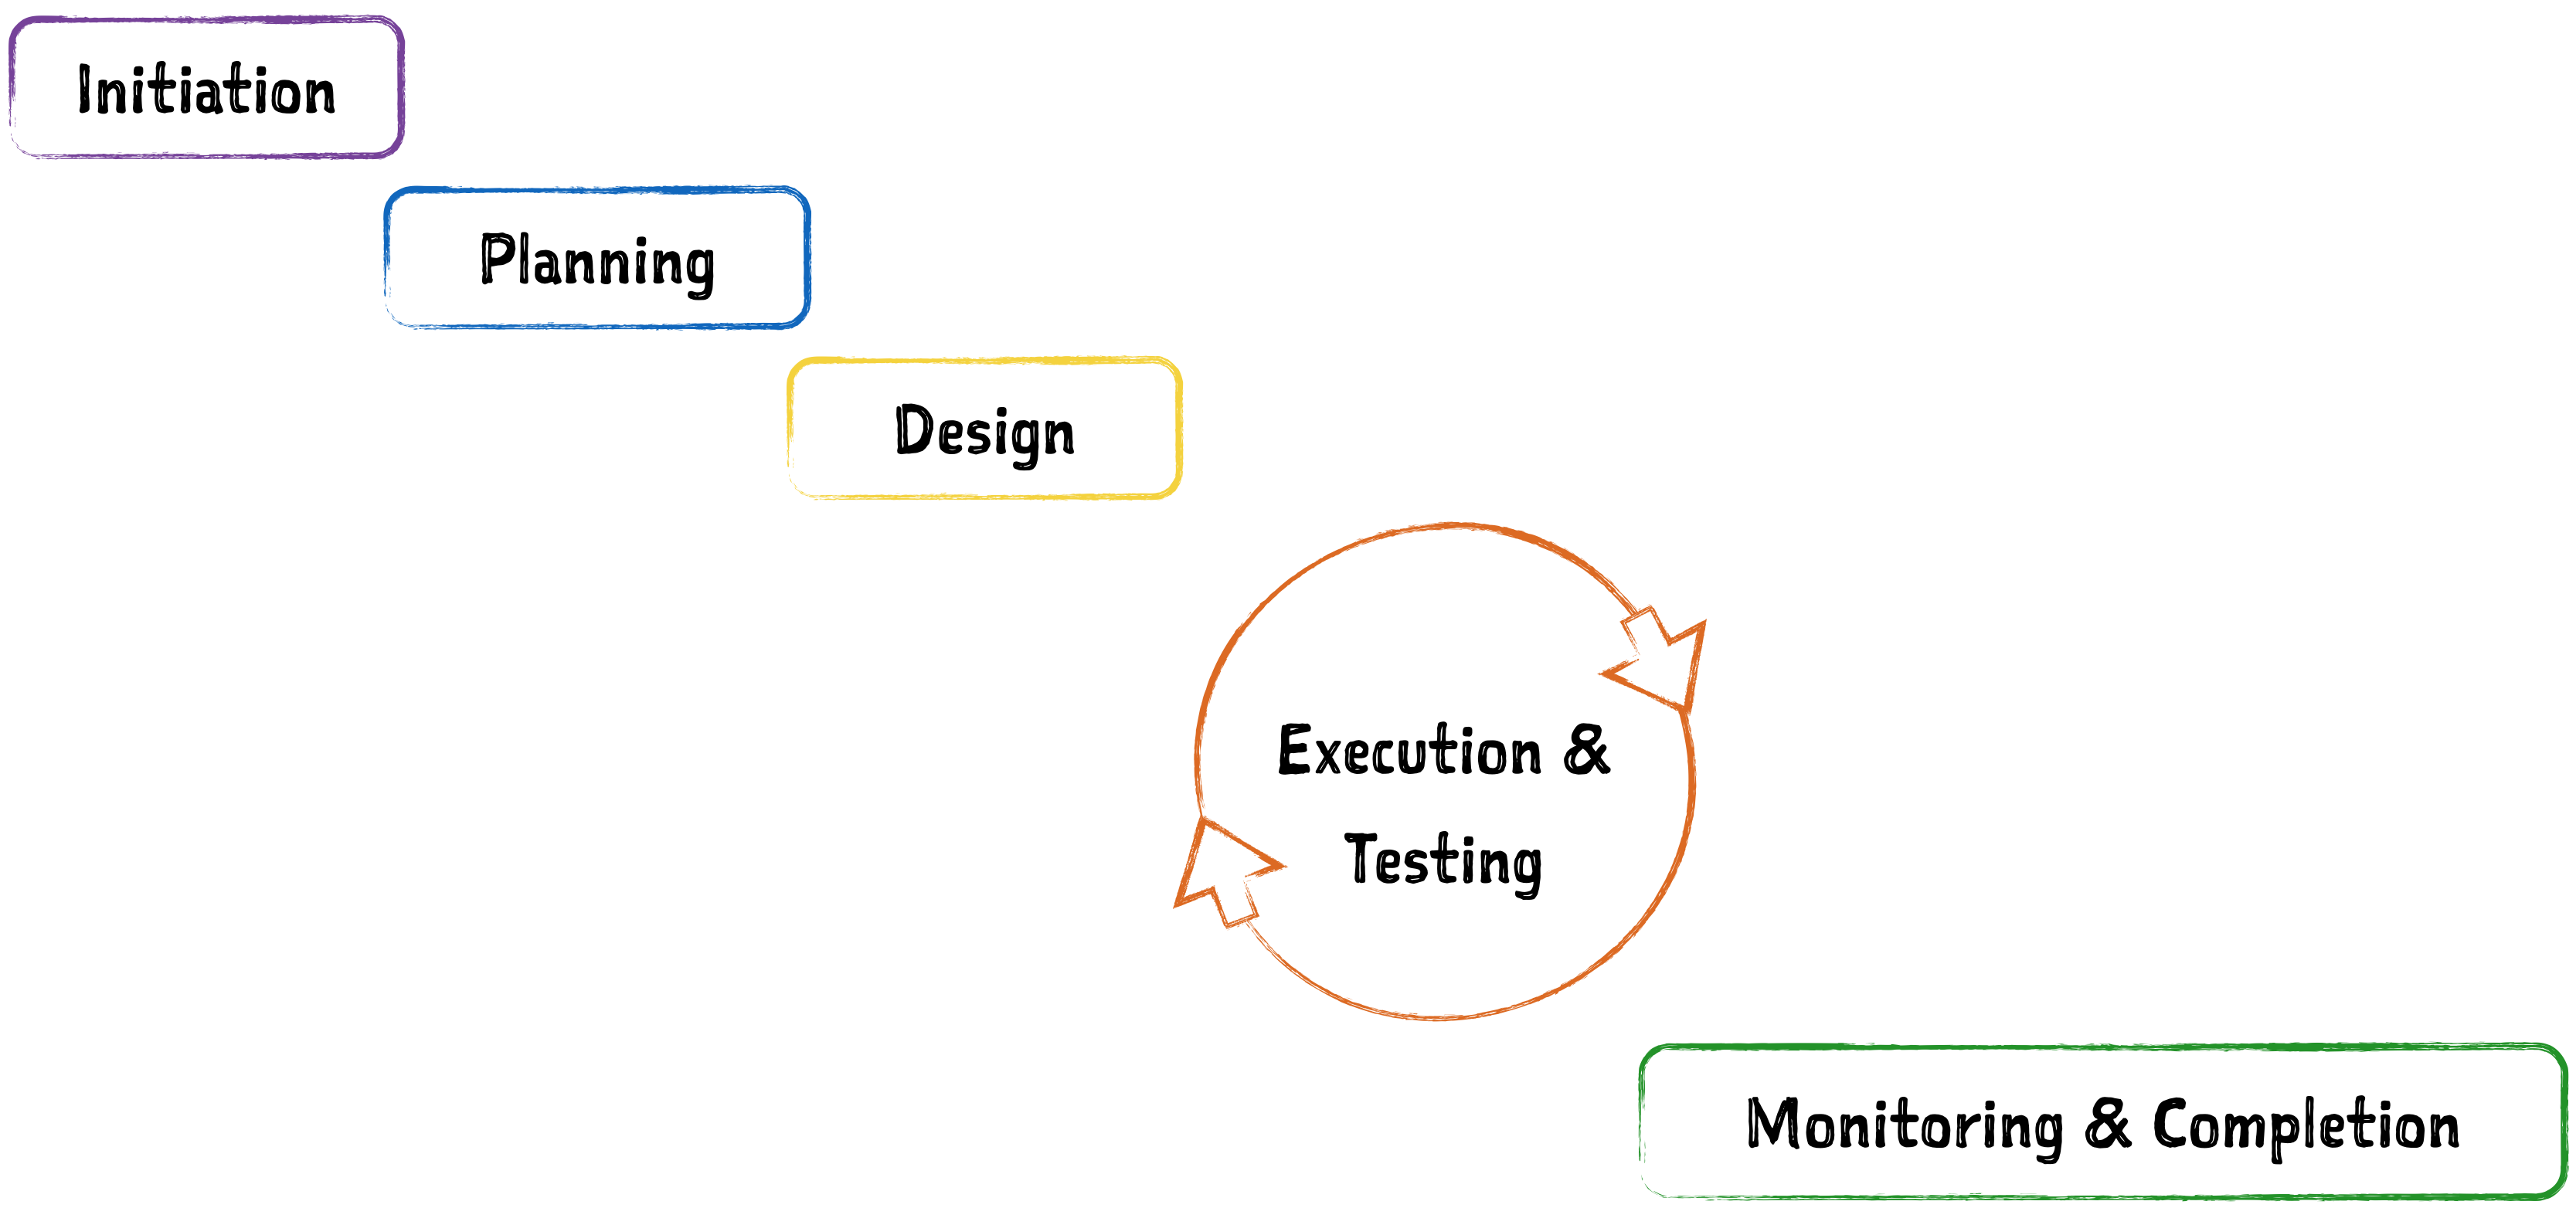
\includegraphics[scale=0.25]{proj_phases}
	\caption{مسیر پروژه}
	\label{phases} % Unique label used for referencing the figure in-text
	%\addcontentsline{toc}{figure}{Figure \ref{fig:placeholder}} % Uncomment to add the figure to the table of contents
\end{figure}

\pagebreak
\section{تحویل‌دادنی‌ها}
تحویل‌دادنی‌های هر فاز از پروژه به‌صورت زیر خواهد بود:

\begin{itemize}
	\item 
	فاز اول
	\subitem
	پیشنهادنامه‌ی پروژه (پروپوزال)
	\subitem نمودار گنت \LTRfootnote{Gantt Chart}
	\subitem نمودار پرت \LTRfootnote{Pert Chart}
	\item 
	فاز دوم
	\subitem  بنمودار مورد استفاده

	
	\item 
	فاز سوم
	\subitem نمودار جریان داده‌ها \LTRfootnote{Data flow Diagram}
	\subitem
	نمودار داده رابطه‌ای
	
	\item 
فاز چهارم
	\subitem نسخه‌ی نهایی «دنگ‌»
	\subitem مستندات پروژه
	
	\item 
	فاز پنجم
	
	\subitem گزارش عملکرد محصول
	\subitem گزارش باگ‌های احتمالی
	\subitem گزارش تغییرات اعمال شده در نسخه‌های جدید
\end{itemize}